\documentclass[12pt,a4paper]{article}

\usepackage[a4paper,text={16.5cm,25.2cm},centering]{geometry}
\usepackage{lmodern}
\usepackage{amssymb,amsmath}
\usepackage{bm}
\usepackage{graphicx}
\usepackage{microtype}
\usepackage{hyperref}
\usepackage{mhchem}
\setlength{\parindent}{0pt}
\setlength{\parskip}{1.2ex}

\hypersetup
       {   pdfauthor = { Ashton Bradley },
           pdftitle={ Bright soliton in a 1D ring },
           colorlinks=TRUE,
           linkcolor=black,
           citecolor=blue,
           urlcolor=blue
       }

\title{ Bright soliton in a 1D ring }

\author{ Ashton Bradley }


\usepackage{upquote}
\usepackage{listings}
\usepackage{xcolor}
\lstset{
    basicstyle=\ttfamily\footnotesize,
    upquote=true,
    breaklines=true,
    breakindent=0pt,
    keepspaces=true,
    showspaces=false,
    columns=fullflexible,
    showtabs=false,
    showstringspaces=false,
    escapeinside={(*@}{@*)},
    extendedchars=true,
}
\newcommand{\HLJLt}[1]{#1}
\newcommand{\HLJLw}[1]{#1}
\newcommand{\HLJLe}[1]{#1}
\newcommand{\HLJLeB}[1]{#1}
\newcommand{\HLJLo}[1]{#1}
\newcommand{\HLJLk}[1]{\textcolor[RGB]{148,91,176}{\textbf{#1}}}
\newcommand{\HLJLkc}[1]{\textcolor[RGB]{59,151,46}{\textit{#1}}}
\newcommand{\HLJLkd}[1]{\textcolor[RGB]{214,102,97}{\textit{#1}}}
\newcommand{\HLJLkn}[1]{\textcolor[RGB]{148,91,176}{\textbf{#1}}}
\newcommand{\HLJLkp}[1]{\textcolor[RGB]{148,91,176}{\textbf{#1}}}
\newcommand{\HLJLkr}[1]{\textcolor[RGB]{148,91,176}{\textbf{#1}}}
\newcommand{\HLJLkt}[1]{\textcolor[RGB]{148,91,176}{\textbf{#1}}}
\newcommand{\HLJLn}[1]{#1}
\newcommand{\HLJLna}[1]{#1}
\newcommand{\HLJLnb}[1]{#1}
\newcommand{\HLJLnbp}[1]{#1}
\newcommand{\HLJLnc}[1]{#1}
\newcommand{\HLJLncB}[1]{#1}
\newcommand{\HLJLnd}[1]{\textcolor[RGB]{214,102,97}{#1}}
\newcommand{\HLJLne}[1]{#1}
\newcommand{\HLJLneB}[1]{#1}
\newcommand{\HLJLnf}[1]{\textcolor[RGB]{66,102,213}{#1}}
\newcommand{\HLJLnfm}[1]{\textcolor[RGB]{66,102,213}{#1}}
\newcommand{\HLJLnp}[1]{#1}
\newcommand{\HLJLnl}[1]{#1}
\newcommand{\HLJLnn}[1]{#1}
\newcommand{\HLJLno}[1]{#1}
\newcommand{\HLJLnt}[1]{#1}
\newcommand{\HLJLnv}[1]{#1}
\newcommand{\HLJLnvc}[1]{#1}
\newcommand{\HLJLnvg}[1]{#1}
\newcommand{\HLJLnvi}[1]{#1}
\newcommand{\HLJLnvm}[1]{#1}
\newcommand{\HLJLl}[1]{#1}
\newcommand{\HLJLld}[1]{\textcolor[RGB]{148,91,176}{\textit{#1}}}
\newcommand{\HLJLs}[1]{\textcolor[RGB]{201,61,57}{#1}}
\newcommand{\HLJLsa}[1]{\textcolor[RGB]{201,61,57}{#1}}
\newcommand{\HLJLsb}[1]{\textcolor[RGB]{201,61,57}{#1}}
\newcommand{\HLJLsc}[1]{\textcolor[RGB]{201,61,57}{#1}}
\newcommand{\HLJLsd}[1]{\textcolor[RGB]{201,61,57}{#1}}
\newcommand{\HLJLsdB}[1]{\textcolor[RGB]{201,61,57}{#1}}
\newcommand{\HLJLsdC}[1]{\textcolor[RGB]{201,61,57}{#1}}
\newcommand{\HLJLse}[1]{\textcolor[RGB]{59,151,46}{#1}}
\newcommand{\HLJLsh}[1]{\textcolor[RGB]{201,61,57}{#1}}
\newcommand{\HLJLsi}[1]{#1}
\newcommand{\HLJLso}[1]{\textcolor[RGB]{201,61,57}{#1}}
\newcommand{\HLJLsr}[1]{\textcolor[RGB]{201,61,57}{#1}}
\newcommand{\HLJLss}[1]{\textcolor[RGB]{201,61,57}{#1}}
\newcommand{\HLJLssB}[1]{\textcolor[RGB]{201,61,57}{#1}}
\newcommand{\HLJLnB}[1]{\textcolor[RGB]{59,151,46}{#1}}
\newcommand{\HLJLnbB}[1]{\textcolor[RGB]{59,151,46}{#1}}
\newcommand{\HLJLnfB}[1]{\textcolor[RGB]{59,151,46}{#1}}
\newcommand{\HLJLnh}[1]{\textcolor[RGB]{59,151,46}{#1}}
\newcommand{\HLJLni}[1]{\textcolor[RGB]{59,151,46}{#1}}
\newcommand{\HLJLnil}[1]{\textcolor[RGB]{59,151,46}{#1}}
\newcommand{\HLJLnoB}[1]{\textcolor[RGB]{59,151,46}{#1}}
\newcommand{\HLJLoB}[1]{\textcolor[RGB]{102,102,102}{\textbf{#1}}}
\newcommand{\HLJLow}[1]{\textcolor[RGB]{102,102,102}{\textbf{#1}}}
\newcommand{\HLJLp}[1]{#1}
\newcommand{\HLJLc}[1]{\textcolor[RGB]{153,153,119}{\textit{#1}}}
\newcommand{\HLJLch}[1]{\textcolor[RGB]{153,153,119}{\textit{#1}}}
\newcommand{\HLJLcm}[1]{\textcolor[RGB]{153,153,119}{\textit{#1}}}
\newcommand{\HLJLcp}[1]{\textcolor[RGB]{153,153,119}{\textit{#1}}}
\newcommand{\HLJLcpB}[1]{\textcolor[RGB]{153,153,119}{\textit{#1}}}
\newcommand{\HLJLcs}[1]{\textcolor[RGB]{153,153,119}{\textit{#1}}}
\newcommand{\HLJLcsB}[1]{\textcolor[RGB]{153,153,119}{\textit{#1}}}
\newcommand{\HLJLg}[1]{#1}
\newcommand{\HLJLgd}[1]{#1}
\newcommand{\HLJLge}[1]{#1}
\newcommand{\HLJLgeB}[1]{#1}
\newcommand{\HLJLgh}[1]{#1}
\newcommand{\HLJLgi}[1]{#1}
\newcommand{\HLJLgo}[1]{#1}
\newcommand{\HLJLgp}[1]{#1}
\newcommand{\HLJLgs}[1]{#1}
\newcommand{\HLJLgsB}[1]{#1}
\newcommand{\HLJLgt}[1]{#1}


\begin{document}

\maketitle

\section{Prelude}
First, let's load some packages and set plot defaults.


\begin{lstlisting}
(*@\HLJLk{using}@*) (*@\HLJLn{Plots}@*)(*@\HLJLp{,}@*) (*@\HLJLn{LaTeXStrings}@*)
(*@\HLJLnf{gr}@*)(*@\HLJLp{(}@*)(*@\HLJLn{legend}@*)(*@\HLJLoB{=}@*)(*@\HLJLkc{false}@*)(*@\HLJLp{,}@*)(*@\HLJLn{titlefontsize}@*)(*@\HLJLoB{=}@*)(*@\HLJLni{12}@*)(*@\HLJLp{,}@*)(*@\HLJLn{size}@*)(*@\HLJLoB{=}@*)(*@\HLJLp{(}@*)(*@\HLJLni{500}@*)(*@\HLJLp{,}@*)(*@\HLJLni{300}@*)(*@\HLJLp{),}@*)(*@\HLJLn{colorbar}@*)(*@\HLJLoB{=}@*)(*@\HLJLkc{false}@*)(*@\HLJLp{,}@*)(*@\HLJLn{grid}@*)(*@\HLJLoB{=}@*)(*@\HLJLkc{false}@*)(*@\HLJLp{)}@*)
(*@\HLJLk{using}@*) (*@\HLJLn{FourierGPE}@*)
\end{lstlisting}


\section{Gross-Pitaevskii equation}
We are going to solve the Gross-Pitaevskii equation

\[
i\hbar\frac{\partial \psi(x,t)}{\partial t}=\left(-\frac{\hbar^2\partial_x^2}{2m}+V(x,t)+g|\psi|^2\right)\psi
\]
for particular initial and boundary conditions.

\subsection{Bright soliton}
The bright soliton provides a good test of any numerical simulation of the Gross-Pitaevskii equation as it involves a delicate balance between kinetic dispersion and the attractive nonlinearity. An initial state with finite momentum also tests the periodicity of the fft method since the soliton will eventually wrap around the domain.

The bright soliton wavefunction with wavenumber $k$ describing its collective motion is

\[
\psi_s(x)= \sqrt{\frac{N_s}{2\xi_s}}\textrm{sech}(x/\xi_s)e^{ikx}
\]
where the soliton scale $\xi_s$ for $N_s$ particles is given by

\[
\xi_s \equiv \frac{2}{|g|N_s}
\]
\section{Simulation}
\subsection{Potential function}

\begin{lstlisting}
(*@\HLJLk{import}@*) (*@\HLJLn{FourierGPE}@*)(*@\HLJLoB{.}@*)(*@\HLJLn{V}@*)
(*@\HLJLnf{V}@*)(*@\HLJLp{(}@*)(*@\HLJLn{x}@*)(*@\HLJLp{,}@*)(*@\HLJLn{t}@*)(*@\HLJLp{)}@*) (*@\HLJLoB{=}@*) (*@\HLJLnfB{0.0}@*) (*@\HLJLoB{|>}@*) (*@\HLJLn{complex}@*)
\end{lstlisting}

\begin{lstlisting}
V (generic function with 3 methods)
\end{lstlisting}


\subsection{Units}
In any numerical calculations we should have a clear understanding of our choice of physical units.

In length unit $\xi_s$, and time unit

\[
t_s\equiv \frac{m \xi_s^2}{\hbar},
\]
and rescaled wavefunction $\bar\psi = \psi\sqrt{\xi_s}$, our dimensionless form of the equation of motion is

\[
i\frac{\partial \bar\psi(\bar x,\bar t)}{\partial \bar t}=\left(-\frac{\bar\partial_x^2}{2}+\bar g|\bar\psi|^2\right)\bar\psi
\]
where the dimensionless interaction parameter is

\[
\bar g \equiv \frac{m\xi_s}{\hbar^2}g < 0
\]
\section{Initialize the simulation}
Create the \texttt{sim} struct holding all parameters, with predefined grids.


\begin{lstlisting}
(*@\HLJLn{L}@*) (*@\HLJLoB{=}@*) (*@\HLJLp{(}@*)(*@\HLJLnfB{60.0}@*)(*@\HLJLp{,)}@*)
(*@\HLJLn{N}@*) (*@\HLJLoB{=}@*) (*@\HLJLp{(}@*)(*@\HLJLni{512}@*)(*@\HLJLp{,)}@*)
(*@\HLJLn{sim}@*) (*@\HLJLoB{=}@*) (*@\HLJLnf{Sim}@*)(*@\HLJLp{(}@*)(*@\HLJLn{L}@*)(*@\HLJLp{,}@*)(*@\HLJLn{N}@*)(*@\HLJLp{)}@*)
(*@\HLJLnd{@unpack{\_}Sim}@*) (*@\HLJLn{sim}@*)(*@\HLJLp{;}@*)
\end{lstlisting}


\section{Parameters}

\begin{lstlisting}
(*@\HLJLn{\ensuremath{\mu}}@*) (*@\HLJLoB{=}@*) (*@\HLJLnfB{25.0}@*)
(*@\HLJLn{g}@*) (*@\HLJLoB{=}@*) (*@\HLJLoB{-}@*)(*@\HLJLnfB{0.01}@*)
(*@\HLJLn{\ensuremath{\gamma}}@*) (*@\HLJLoB{=}@*) (*@\HLJLnfB{0.0}@*)
(*@\HLJLn{Ns}@*) (*@\HLJLoB{=}@*) (*@\HLJLni{200}@*)
(*@\HLJLn{\ensuremath{\xi}s}@*) (*@\HLJLoB{=}@*) (*@\HLJLni{2}@*)(*@\HLJLoB{/}@*)(*@\HLJLnf{abs}@*)(*@\HLJLp{(}@*)(*@\HLJLn{g}@*)(*@\HLJLp{)}@*)(*@\HLJLoB{/}@*)(*@\HLJLn{Ns}@*)
(*@\HLJLn{us}@*) (*@\HLJLoB{=}@*) (*@\HLJLni{20}@*)
(*@\HLJLn{tf}@*) (*@\HLJLoB{=}@*) (*@\HLJLni{1}@*)(*@\HLJLn{\ensuremath{\pi}}@*) (*@\HLJLoB{|>}@*) (*@\HLJLn{Float64}@*)
(*@\HLJLn{Nt}@*) (*@\HLJLoB{=}@*) (*@\HLJLni{150}@*)
(*@\HLJLn{t}@*) (*@\HLJLoB{=}@*) (*@\HLJLnf{LinRange}@*)(*@\HLJLp{(}@*)(*@\HLJLnfB{0.}@*)(*@\HLJLp{,}@*)(*@\HLJLn{tf}@*)(*@\HLJLp{,}@*)(*@\HLJLn{Nt}@*)(*@\HLJLp{);}@*)
\end{lstlisting}


\subsection{Initial condition}
We initialize the bright soliton with dimensionless velocity $u_s$ as


\begin{lstlisting}
(*@\HLJLn{x}@*) (*@\HLJLoB{=}@*) (*@\HLJLn{X}@*)(*@\HLJLp{[}@*)(*@\HLJLni{1}@*)(*@\HLJLp{]}@*)
(*@\HLJLnf{\ensuremath{\psi}s}@*)(*@\HLJLp{(}@*)(*@\HLJLn{x}@*)(*@\HLJLp{)}@*) (*@\HLJLoB{=}@*) (*@\HLJLnf{sqrt}@*)(*@\HLJLp{(}@*)(*@\HLJLn{Ns}@*)(*@\HLJLoB{/}@*)(*@\HLJLni{2}@*)(*@\HLJLn{\ensuremath{\xi}s}@*)(*@\HLJLp{)}@*)(*@\HLJLoB{*}@*)(*@\HLJLnf{sech}@*)(*@\HLJLp{(}@*)(*@\HLJLn{x}@*)(*@\HLJLoB{/}@*)(*@\HLJLn{\ensuremath{\xi}s}@*)(*@\HLJLp{)}@*)(*@\HLJLoB{*}@*)(*@\HLJLnf{exp}@*)(*@\HLJLp{(}@*)(*@\HLJLn{im}@*)(*@\HLJLoB{*}@*)(*@\HLJLn{us}@*)(*@\HLJLoB{*}@*)(*@\HLJLn{x}@*)(*@\HLJLp{)}@*)
(*@\HLJLn{\ensuremath{\psi}i}@*) (*@\HLJLoB{=}@*) (*@\HLJLn{\ensuremath{\psi}s}@*)(*@\HLJLoB{.}@*)(*@\HLJLp{(}@*)(*@\HLJLn{x}@*)(*@\HLJLp{)}@*)
(*@\HLJLn{\ensuremath{\phi}i}@*) (*@\HLJLoB{=}@*) (*@\HLJLnf{kspace}@*)(*@\HLJLp{(}@*)(*@\HLJLn{\ensuremath{\psi}i}@*)(*@\HLJLp{,}@*)(*@\HLJLn{sim}@*)(*@\HLJLp{)}@*)

(*@\HLJLnd{@pack{\_}Sim!}@*) (*@\HLJLn{sim}@*)(*@\HLJLp{;}@*) (*@\HLJLcs{{\#}finally,}@*) (*@\HLJLcs{pack}@*) (*@\HLJLcs{everything}@*) (*@\HLJLcs{up}@*) (*@\HLJLcs{for}@*) (*@\HLJLcs{simulation.}@*)
\end{lstlisting}


\subsection{Evolve in k-space}
Now we have everything we need to evolve in k-space


\begin{lstlisting}
(*@\HLJLnd{@time}@*) (*@\HLJLn{sol}@*) (*@\HLJLoB{=}@*) (*@\HLJLnf{runsim}@*)(*@\HLJLp{(}@*)(*@\HLJLn{sim}@*)(*@\HLJLp{);}@*)
\end{lstlisting}

\begin{lstlisting}
4.387429 seconds (8.46 M allocations: 543.949 MiB, 1.91(*@{{\%}}@*) gc time, 31.50(*@{{\%}}@*) 
compilation time)
\end{lstlisting}


\subsection{Plot the solution}
We plot the density of atoms, and the phase after removing the Galilean boost.


\begin{lstlisting}
(*@\HLJLn{\ensuremath{\psi}p}@*) (*@\HLJLoB{=}@*) (*@\HLJLnf{xspace}@*)(*@\HLJLp{(}@*)(*@\HLJLn{sol}@*)(*@\HLJLp{[}@*)(*@\HLJLk{end}@*)(*@\HLJLp{],}@*)(*@\HLJLn{sim}@*)(*@\HLJLp{)}@*)(*@\HLJLoB{.*}@*)(*@\HLJLn{exp}@*)(*@\HLJLoB{.}@*)(*@\HLJLp{(}@*)(*@\HLJLoB{-}@*)(*@\HLJLn{im}@*)(*@\HLJLoB{*}@*)(*@\HLJLn{us}@*)(*@\HLJLoB{*}@*)(*@\HLJLn{x}@*)(*@\HLJLp{)}@*)
(*@\HLJLn{p1}@*) (*@\HLJLoB{=}@*) (*@\HLJLnf{plot}@*)(*@\HLJLp{(}@*)(*@\HLJLn{x}@*)(*@\HLJLp{,}@*)(*@\HLJLn{abs2}@*)(*@\HLJLoB{.}@*)(*@\HLJLp{(}@*)(*@\HLJLn{\ensuremath{\psi}p}@*)(*@\HLJLp{))}@*)
(*@\HLJLnf{xlabel!}@*)(*@\HLJLp{(}@*)(*@\HLJLso{L"{}x"{}}@*)(*@\HLJLp{);}@*)(*@\HLJLnf{ylabel!}@*)(*@\HLJLp{(}@*)(*@\HLJLso{L"{}|{\textbackslash}psi|{\textasciicircum}2"{}}@*)(*@\HLJLp{)}@*)
(*@\HLJLn{p2}@*) (*@\HLJLoB{=}@*) (*@\HLJLnf{plot}@*)(*@\HLJLp{(}@*)(*@\HLJLn{x}@*)(*@\HLJLp{,}@*)(*@\HLJLn{angle}@*)(*@\HLJLoB{.}@*)(*@\HLJLp{(}@*)(*@\HLJLn{\ensuremath{\psi}p}@*)(*@\HLJLp{))}@*)
(*@\HLJLnf{xlabel!}@*)(*@\HLJLp{(}@*)(*@\HLJLso{L"{}x"{}}@*)(*@\HLJLp{);}@*)(*@\HLJLnf{ylabel!}@*)(*@\HLJLp{(}@*)(*@\HLJLso{L"{}{\textbackslash}textrm{\{}phase{\}}}@*) (*@\HLJLso{({\textbackslash}psi)"{}}@*)(*@\HLJLp{)}@*)
(*@\HLJLn{p}@*) (*@\HLJLoB{=}@*) (*@\HLJLnf{plot}@*)(*@\HLJLp{(}@*)(*@\HLJLn{p1}@*)(*@\HLJLp{,}@*)(*@\HLJLn{p2}@*)(*@\HLJLp{,}@*)(*@\HLJLn{layout}@*)(*@\HLJLoB{=}@*)(*@\HLJLp{(}@*)(*@\HLJLni{2}@*)(*@\HLJLp{,}@*)(*@\HLJLni{1}@*)(*@\HLJLp{),}@*)(*@\HLJLn{size}@*)(*@\HLJLoB{=}@*)(*@\HLJLp{(}@*)(*@\HLJLni{600}@*)(*@\HLJLp{,}@*)(*@\HLJLni{400}@*)(*@\HLJLp{))}@*)
\end{lstlisting}

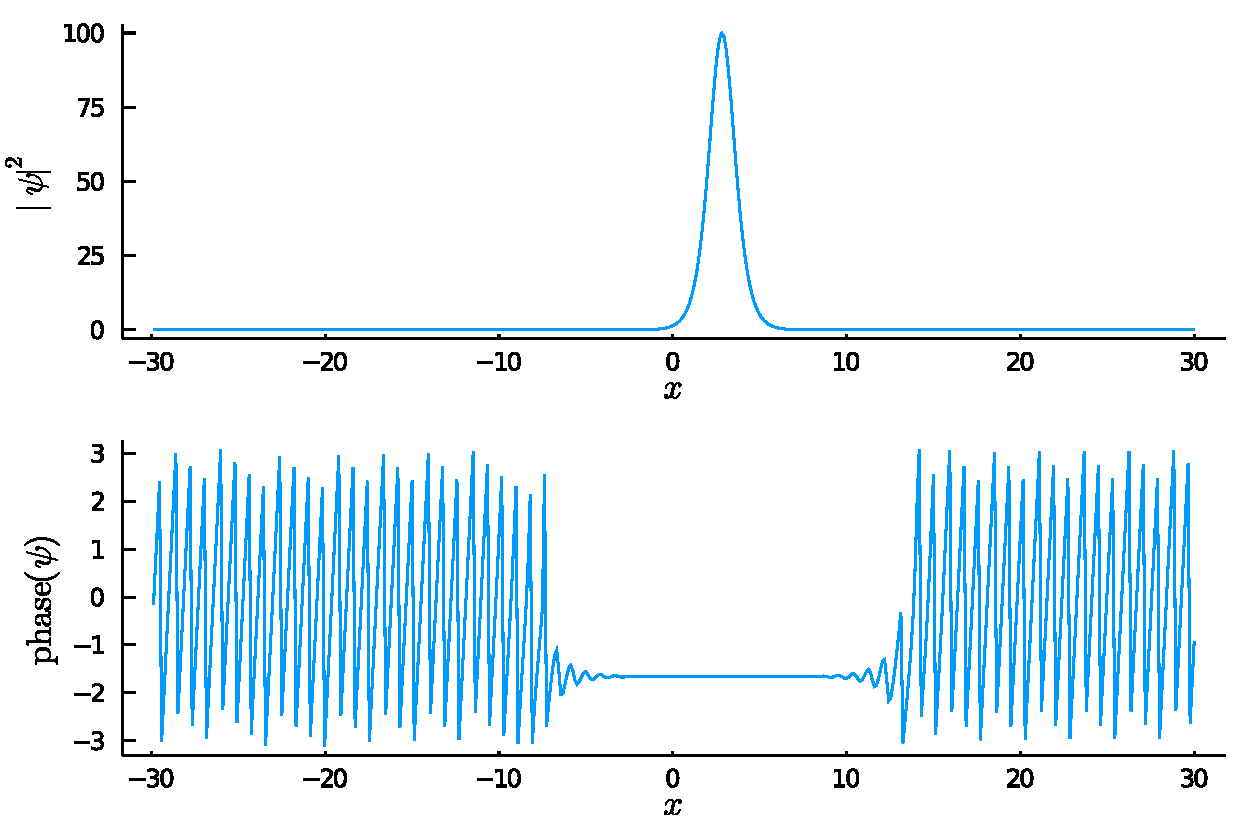
\includegraphics[width=\linewidth]{jl_EXlQxb/1dbrightsoliton_7_1.pdf}

The phase is constant over the soliton, as it would be in the lab frame.  To visualize the motion, we can make an animation, saved to the \href{../../media/brightsoliton.gif}{media folder}.


\begin{lstlisting}
(*@\HLJLn{anim}@*) (*@\HLJLoB{=}@*) (*@\HLJLnd{@animate}@*) (*@\HLJLk{for}@*) (*@\HLJLn{i}@*)(*@\HLJLoB{=}@*)(*@\HLJLni{1}@*)(*@\HLJLoB{:}@*)(*@\HLJLn{Nt}@*)(*@\HLJLoB{-}@*)(*@\HLJLni{8}@*)
    (*@\HLJLn{\ensuremath{\psi}}@*) (*@\HLJLoB{=}@*) (*@\HLJLnf{xspace}@*)(*@\HLJLp{(}@*)(*@\HLJLn{sol}@*)(*@\HLJLp{[}@*)(*@\HLJLn{i}@*)(*@\HLJLp{],}@*)(*@\HLJLn{sim}@*)(*@\HLJLp{)}@*)
    (*@\HLJLn{y}@*) (*@\HLJLoB{=}@*) (*@\HLJLn{abs2}@*)(*@\HLJLoB{.}@*)(*@\HLJLp{(}@*)(*@\HLJLn{\ensuremath{\psi}}@*)(*@\HLJLp{)}@*)
    (*@\HLJLnf{plot}@*)(*@\HLJLp{(}@*)(*@\HLJLn{x}@*)(*@\HLJLp{,}@*)(*@\HLJLn{y}@*)(*@\HLJLp{,}@*)(*@\HLJLn{fill}@*)(*@\HLJLoB{=}@*)(*@\HLJLp{(}@*)(*@\HLJLni{0}@*)(*@\HLJLp{,}@*) (*@\HLJLnfB{0.2}@*)(*@\HLJLp{),}@*)(*@\HLJLn{size}@*)(*@\HLJLoB{=}@*)(*@\HLJLp{(}@*)(*@\HLJLni{600}@*)(*@\HLJLp{,}@*)(*@\HLJLni{150}@*)(*@\HLJLp{),}@*)(*@\HLJLn{legend}@*)(*@\HLJLoB{=}@*)(*@\HLJLkc{false}@*)(*@\HLJLp{,}@*)(*@\HLJLn{xticks}@*)(*@\HLJLoB{=}@*)(*@\HLJLkc{false}@*)(*@\HLJLp{,}@*)(*@\HLJLn{yticks}@*)(*@\HLJLoB{=}@*)(*@\HLJLkc{false}@*)(*@\HLJLp{,}@*)(*@\HLJLn{axis}@*)(*@\HLJLoB{=}@*)(*@\HLJLkc{false}@*)(*@\HLJLp{)}@*)
(*@\HLJLk{end}@*)

(*@\HLJLn{filename}@*) (*@\HLJLoB{=}@*) (*@\HLJLs{"{}brightsoliton.gif"{}}@*)
(*@\HLJLnf{gif}@*)(*@\HLJLp{(}@*)(*@\HLJLn{anim}@*)(*@\HLJLp{,}@*)(*@\HLJLnf{joinpath}@*)(*@\HLJLp{(}@*)(*@\HLJLnd{@{\_}{\_}DIR{\_}{\_}}@*)(*@\HLJLp{,}@*)(*@\HLJLs{"{}../media"{}}@*)(*@\HLJLp{,}@*)(*@\HLJLn{filename}@*)(*@\HLJLp{),}@*)(*@\HLJLn{fps}@*) (*@\HLJLoB{=}@*) (*@\HLJLni{25}@*)(*@\HLJLp{);}@*)
\end{lstlisting}


\begin{figure}
\centering
\includegraphics{../../media/brightsoliton.gif}
\caption{[animation (see media folder)]}
\end{figure}




\end{document}
